% ===================================
% CODICE LaTeX PER GRAFICI E TABELLE
% Tesi GDO - Capitoli 1 e 2
% ===================================
% filepath: c:\Users\saint\tesi\nuovi grafi 1 e 2.tex
\documentclass[border=10pt]{standalone}
% Pacchetti necessari

\usepackage[T1]{fontenc}
\usepackage{amsmath}
\usepackage{amssymb}    
\usepackage{graphicx}
\usepackage{caption}
\usepackage{subcaption} % Per sottotitoli nelle figure
% Preambolo necessario:
\usepackage{tikz}
\usepackage{pgfplots}
\usepackage{booktabs}
\usepackage{multirow}
\pgfplotsset{compat=1.17}
\usetikzlibrary{pgfplots.polar}

% ===================================
% CAPITOLO 1
% ===================================
\begin{document}
% FIGURA 1.1: Gap tra Ricerca e Implementazione

\centering
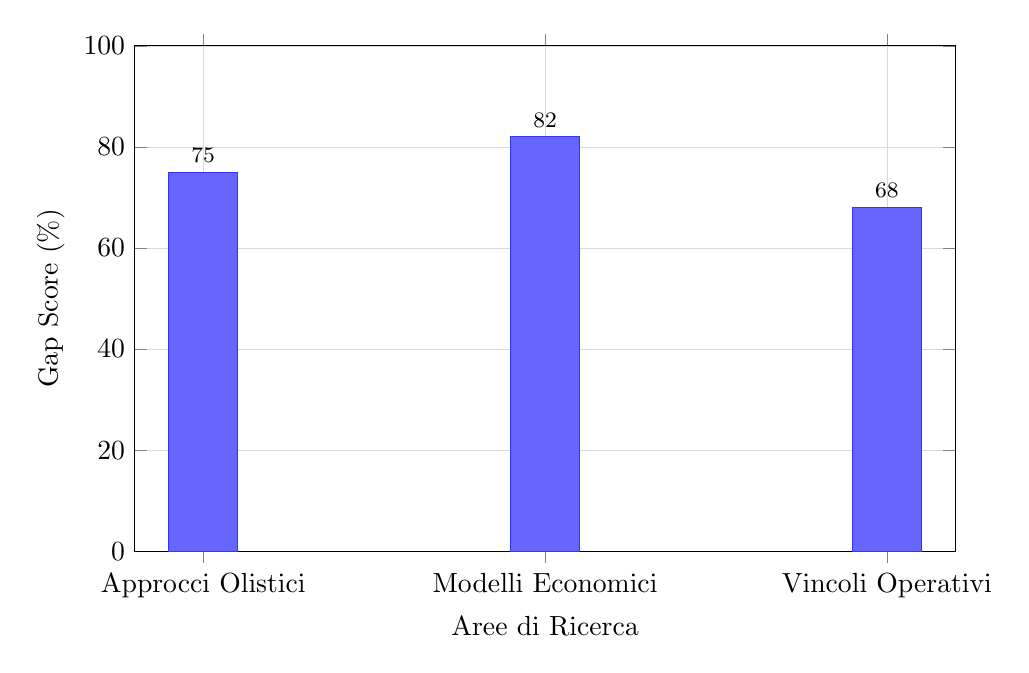
\begin{tikzpicture}
\begin{axis}[
    ybar,
    width=12cm,
    height=8cm,
    ylabel={Gap Score (\%)},
    xlabel={Aree di Ricerca},
    symbolic x coords={Approcci Olistici,Modelli Economici,Vincoli Operativi},
    xtick=data,
    ymin=0,
    ymax=100,
    bar width=25pt,
    nodes near coords,
    every node near coord/.append style={font=\footnotesize},
    grid=major,
    grid style={line width=.1pt, draw=gray!30},
    legend style={at={(0.5,-0.15)},anchor=north}
]
\addplot[fill=blue!60, draw=blue!80] coordinates {
    (Approcci Olistici,75)
    (Modelli Economici,82)
    (Vincoli Operativi,68)
};
\end{axis}
\end{tikzpicture}
\end{document}

